\documentclass[11pt,a4paper]{article}

% Arial
\usepackage{helvet}
\renewcommand{\familydefault}{\sfdefault}

% 1.5 distance between lines
\linespread{1.5}

% reduce those generous margins a bit
\usepackage[hmargin=3.5cm,vmargin=3cm]{geometry}

% keep the text clean
\usepackage[fleqn]{nccmath}
\usepackage{enumitem}
\setlist[itemize]{noitemsep}
\setdescription{leftmargin=\parindent,labelindent=1cm}
\usepackage[parfill]{parskip}

% Be able to link urls
\usepackage{hyperref}

% Hide the ugly url border
\hypersetup{
    colorlinks=true,        % false: boxed links; true: colored links
    linkcolor=black,        % color of internal links (change box color with linkbordercolor)
    citecolor=green,        % color of links to bibliography
    filecolor=magenta,      % color of file links
    urlcolor=cyan,          % color of external links
    pdfborder={0 0 0},
}

% pgfplots for more complex stuff
\usepackage{pgfplots}
\usetikzlibrary{arrows}
\pagestyle{empty}

% Images
\usepackage{graphicx}

% Bibliography
\bibliographystyle{acm}

% Wrapping for figures
\usepackage{wrapfig}

% Java source code support
\usepackage{listings}
\usepackage{color}
\definecolor{dkgreen}{rgb}{0,0.6,0}
\definecolor{gray}{rgb}{0.5,0.5,0.5}
\definecolor{mauve}{rgb}{0.58,0,0.82}
\lstset{frame=tb,
  language=Java,
  aboveskip=3mm,
  belowskip=3mm,
  showstringspaces=false,
  columns=flexible,
  basicstyle={\linespread{0.8}\small\ttfamily},
  numbers=none,
  numberstyle=\tiny\color{gray},
  keywordstyle=\color{blue},
  commentstyle=\color{dkgreen},
  stringstyle=\color{mauve},
  breaklines=true,
  breakatwhitespace=true
  tabsize=4
}

% Define floor
\providecommand{\floor}[1]{\left \lfloor #1 \right \rfloor }

% Math stuff
\usepackage{amsmath}

% Title
\title{\LARGE \textbf {Programming a Modular Software Synthesizer} \vspace{1em}}
\author{Alexander Liebend\"{o}rfer}

% Document
\begin{document}
\maketitle
\clearpage
\tableofcontents

\clearpage

\section{Preface}

It was never in doubt for me that my ideal matura project would be a software, and from there only a small amount of tasks were simultaneously of my skill level, part of my interests and of the size required for a matura project. Having dabbled in electronic music production before, I was already familiar with the main methods and problems, and was very interested in the precise mathematics. Particularly one software, ZynAddSubFX~\cite{ZASF}, fascinated me by its power, its sound and the shear amount of parameters and control it gave. It was perfect in almost every aspect except for one central flaw which marred it in my opinion, and that was the lack of rewiring support. The sound pipeline was fixed, only a select few parameters could be automated, and those usually did not correspond to what I needed. With this project I hoped to do the opposite, and provided modularity from the ground up. Another goal was to gain an understanding in signal theory, which is best done by creating a project that relied on it. The final choice concerned the programming language, and on advice I chose a language I did not know so well at the time with hopes of learning it; Java.


\section{Introduction}

\subsection{A short history of synthesizers}

A synthesizer is an (usually electronic) device where one can shape and create a sound, normally for use in music. The earliest example that could be considered a synthesizer is a standard pipe organ, as the organ player has a large control over the shape of the sound by choosing what pipes are used. In fact, the organ was even a model for one of the first approaches to synthesis called \emph{additive synthesis}. The basic idea behind additive synthesis is to sum many simple waves together to form a more complex one. This was famously used in an electronic form first by Thaddeus Cahill as the Telharmonium in 1897~\cite{Telharmonium}, and later in smaller, more practical versions like the Hammond organ~\cite{Hammond}.
In the late 1960s a new device named after it's creator Robert Moog appeared and quickly gained fame, as it used a new synthesis paradigm allowing many new sounds to be created. Moog synthesizers used \emph{subtractive synthesis}, in which a sound is first created by summing simple waveforms and then unwanted frequencies are cut out and filtered, to shape the sound in a distinctive way. On top of this, the invention of the transistor just prior made the machine much cheaper and smaller. Since then, different models of the original Moog synthesizer were created, and later competitors joined into what was becoming a large market. More synthesis methods were invented, although subtractive synthesis still is the dominant model to this day thanks to it's simplicity and power, on par with sampling-based techniques. More recently, thanks to the computer, most electronic music is now done digitally with software, as this is again a good deal cheaper and more practical. Professional audio software still can cost large amounts, but usually less so than a full hardware setup, especially including all advantages software brings (plugins, easy distribution, saving, undo/redo, etc).

\subsection{Modularity}

The first analog synthesizers were very modular. One didn't buy "a synthesizer", one bought a few oscillators, 2 or 3 amplifiers, some distortion modules and a lot of cables. These boxes were then placed in racks and connected together in various ways. Even when synthesizers started to be selled as a unit (Moog synthesizer), the ability to freely connect any part with any other on one hand allowed a large amount of freedom and on the other forced the musician to understand the workings of the synthesizer modules themselves~\cite{ModularMoog}. With time, this changed, with the extreme appearing in current software synthesizers, which for the most part only allow the user to modify some parameters, and not the wiring or order of the modules processed. There of course exist exceptions to this rule (Reason is a notable synthesizer which allows changing the wiring, but it is far from absolutely modular~\cite{Reason}), but most famous synthesizers have a fixed pipeline or limited parameter wiring, and none of the well-known professional tools allow custom feedback loops.

\section{Tools}

The only physical tools used were a computer with peripherals, and a sound system. Several software tools were used though, and I will briefly discuss the most important ones here.

The software itself is programmed in Java~\cite{Java}, and hence is dependent of the Java runtime environment (JRE) and all it's requirements. As interface between my software and the OS sound system I used the standard Java Sound API~\cite{Javasound}. The GUI itself was made through a popular GUI package called Swing~\cite{Swing}, which is also used in many professional applications.

On top of the tools directly implicated in the making of the software, a few additional ones were used to fac‎ilitate it. A rather famous IDE named Eclipse~\cite{Eclipse} was used for all Java programming, and of enormous importance was the version control system Git~\cite{Git} (with a few extra features from the webservice Github~\cite{Github}). Python~\cite{Python} and~\cite{Veusz} were slightly used for debugging and graphing purposes, especially for displaying sound output as an image, but have no direct part in the software.

Finally, this text was created with LaTeX~\cite{Latex} and the TikZ/PGF~\cite{Tikz} graphing package for all graphs. Certain parts were created with help of the geometry package Geogebra~\cite{Geogebra}, but were always modified afterwards.

\clearpage

\section{Implementation}

\subsection{Pipes and Modules}

To achieve a completely modular synthesizer, we already need to give up a fixed circuit and have to use the module concept. On top of that, because of recursive loops, we need to actually let the data flow between the different modules, and not just sum the effects of the modules recursively. This means we need at least 1 buffer between every module. We also need a clear way to connect those modules, so a pipe system for connecting inputs and outputs of different modules will be necessary. And finally, some way to inject the current MIDI data and duration of every note as well as a way to capture the processed sound for output is needed.

\subsubsection{Basic system}

In this specific implementation, modules are pure functions, or atleast behave as such towards the outside. A module is always connected to other modules via so-called pipes, which contain the actual data. Modules can then load the data from their input pipes, process it, and dump the result into their output pipes. The main advantage of this system is that it's stable and will work with any wiring setup, even feedback loops. In such closed feedback systems, there will be a propagation delay depending on the amount of pipes the data has to travel, and so no infinite recursion appears. Splitting data and doing parallel processing before merging it again is also implicitely supported, as every module and pipe only acts locally.
One major issue is execution order. A recursive "pull" query where every module calls the modules it depends on for their output cannot work, infinite recursion is a possibility. Even without recursion, there is always the risk that some part of the circuit did not get updated, which might affect the rest. I haven't found a clean solution to this without drawbacks, the one I chose just makes every module execute once in more or less random order (it is not truely random, in fact it is in order of creation), which in worse case causes a signal to wait an extra frame between two modules but guarantees that every module is executed once and only once per frame, and done so in a consistent way.

Injection of user input and retrieval of the sound output is best done with modules dedicated to that. These modules possess only 1 input or output port respectively, and do not by themselves do anything. They just serve as convienient place to connect pipes to, and the main overarching engine can simply read and write the contents of their pipes.

\subsubsection{Dealing with Time}

A tricky problem is dealing with time-sensitive modules, like envelopes or oscillators. The input does not implicitely declare it's duration, so there needs to be a way for the pipes to also carry starting time of a signal. For this, I implemented a separate counter in every pipe, which showed the time at which that signal started. When a module is done with processing and copies the signal data into its output, it also copies in the counter. A negative time can be used as a marker that the pipe is inactive and that module doesn't even need to process anything. Every module can define a special pipe which is taken as reference for the source time, which is especially important when conflicts are possible. If a module does not define such a pipe, the highest starting time (the most recent signal) of all input pipes is assumed to be the reference.

\subsubsection{Stereo/Mono and Polyphony support}

Making one sound is nice, but for making anything remotely musical one must be able to play several sounds at once. Infinite simultaneous sounds would be ideal, but is technically impossible. A number of different channels though, usually around 8 or 16, is simple to implement. Every sound buffer in the pipe is transformed into an array of buffers, and the starting time is transformed into an array. Modules then just iterate between all channels and behave normally for each pipe.
Additionally, a nice feature would be stereo support. My implementation lacks stereo support in the java api calls and the gui, but the engine itself and all the modules and pipes can use stereo. For that, all buffers across all channels are duplicated, to be calculated separately. In fact, there is little difference between stereo and a second layer of channels for polyphony, and so it is treated much the same way.

\subsection{Oscillators}

Oscillators are generators that can create a periodic waveform. They are the basis of additive and subtractive synthesis by creating a basic wave to be shaped and modified by every other module. Usually osillators create a few types of mathematically well-defined primitive waveforms, like sine or square waves. Apart from the wave function, they also possess two parameters, frequency and phase. Frequency describes the amount of oscillations per second, and a difference in frequency is percieved as a difference in pitch. Phase is very difficult to percieve audibly in most cases, it is the initial offset the oscillation started with. Contrarily to frequency, phase has a bounded range, usually from 0 to 2$\pi$ or from 0 to 1, depending on the implementation.

In this synthesizer, the 3 most fundamental waveforms are supported. These are the sine wave, the "square wave" or pulse wave, and the popular sawtooth-wave, also called saw-wave.
\begin{figure}[h]
\caption{Common basic waveforms}
\centering
\resizebox{\textwidth}{!}{
    % Sine wave
    \begin{tikzpicture}[line cap=round,line join=round,>=triangle 45,x=1.0cm,y=1.0cm]
    \draw[->,color=black] (-1,0) -- (18,0);
    \foreach \x in {-1,1,2,3,4,5,6,7,8,9,10,11,12,13,14,15,16,17}
    \draw[shift={(\x,0)},color=black] (0pt,-2pt);
    \draw[->,color=black] (0,-2) -- (0,2);
    \foreach \y in {-2,-1,1}
    \draw[shift={(0,\y)},color=black] (2pt,0pt) -- (-2pt,0pt);
    \clip(-1,-2) rectangle (18,2);
    \draw[smooth,color=blue,samples=100,domain=-1.0:18.0] plot(\x,{sin(((\x))*180/pi)});
    \node [above] at (2,1) {\large Sine wave};
    \end{tikzpicture}
}
\resizebox{\textwidth}{!}{
    % Square wave
    \begin{tikzpicture}[line cap=round,line join=round,>=triangle 45,x=1.0cm,y=1.0cm]
    \draw[->,color=black] (-1,0) -- (18,0);
    \foreach \x in {-1,1,2,3,4,5,6,7,8,9,10,11,12,13,14,15,16,17,18}
    \draw[shift={(\x,0)},color=black] (0pt,-2pt);
    \draw[->,color=black] (0,-2) -- (0,2);
    \foreach \y in {-2,-1,1,2}
    \draw[shift={(0,\y)},color=black] (2pt,0pt) -- (-2pt,0pt);
    \clip(-1,-2) rectangle (18,2);
    \foreach \k in {-1,1,...,17} {
        \def\u{\k*3.141592653589793 - 0.5};
        \draw [color=blue] (\u,-1) -- (\u+3.141592653589793,-1);
        \draw [color=blue] (\u,1) -- (\u,-1);
    }
    \foreach \k in {0,2,...,18} {
        \def\u{\k*3.141592653589793 - 0.5};
        \draw [color=blue] (\u,1) -- (\u+3.141592653589793,1);
        \draw [color=blue] (\u,1) -- (\u,-1);
    }
    \node [above] at (2,1) {\large Square wave};
    \end{tikzpicture}
}
\resizebox{\textwidth}{!}{
    % Saw wave
    \begin{tikzpicture}[line cap=round,line join=round,>=triangle 45,x=1.0cm,y=1.0cm]
    \draw[->,color=black] (-1,0) -- (18,0);
    \foreach \x in {-1,1,2,3,4,5,6,7,8,9,10,11,12,13,14,15,16,17,18}
    \draw[shift={(\x,0)},color=black] (0pt,-2pt);
    \draw[->,color=black] (0,-2) -- (0,2);
    \foreach \y in {-2,-1,1,2}
    \draw[shift={(0,\y)},color=black] (2pt,0pt) -- (-2pt,0pt);
    \clip(-1,-2) rectangle (18,2);
    \foreach \k in {-1,...,18} {
        \def\u{\k*3.141592653589793 - 0.5};
        \draw [color=blue] (\u,-1) -- (\u+3.141592653589793,1);
        \draw [color=blue] (\u,1) -- (\u,-1);
    }
    \node [above] at (2,1) {\large Saw wave};
    \end{tikzpicture}
}
\end{figure}

\subsubsection{Basic implementation}

As already noted, oscillators only require two parameters, phase and frequency. It is quite easy to deal with stereo behavior, as the channels are independent, one can simply first calculate the left side and then the right side. Oscillators also depend heavily on the global time and on the pipe starting time. Through this the current time since starting to oscillate can be calculated trivially, and it is generally a good idea to do modulo the period of the wave as well. Afterwards, the resulting signal is calculated differently depending on the type.
\\\begin{minipage}{\linewidth}
\begin{lstlisting}
double x = time * frequency + phase;
switch (osc_type)
{
	case SINE_WAVE:
		return Math.sin(x*2*Math.PI);

	case SQUARE_WAVE:
		if (x <= 0.5)
		{
		    return 1;
		}
		else
		{
		    return -1;
		}

	case SAW_WAVE:
		return 2*(x - Math.floor(x)) - 1;
}
\end{lstlisting}
\end{minipage}

\subsubsection{Anti-Aliased implementation}

The previous approach worked fine for sine waves, but in both other waveforms there is a regular discontinuity. In the frequency range, this translates to an infinite frequency, inducing aliasing, as the Nyquist frequency cannot be infinite.
There are many, many approaches to fixing this problem in general, it is a recurring obstacle in everything from 3D-graphics to font rendering, and it affects synthesis as well. Luckily, the two waveforms we need are special; their frequencies are easily represented as infinite sums. On top of that, we do not need a particularly fast solution, so we can settle for a mathematically simple and complete one.

The saw wave, in the frequency domain, is nothing but the sum of every harmonic (whole-number multiples of the base frequency) with a 1/k decaying amplitude~\cite{WolframSaw}.
(\(f = \) the base frequency, \(F_N = \) the Nyquist frequency)
\begin{equation}
H(f) = \frac{2}{\pi}\sum\limits_{k=1}^\infty{\frac{\sin(k*f)}{k}}
\end{equation}
\footnote{The \(\frac{2}{\pi}\) normalises the result between -1 and 1.}

Of course, instead of summing to infinity, we could stop summing as soon as \(k*f > F_N\), therefore only including overtones under the Nyquist frequency.
\begin{equation}
H(f) = \frac{2}{\pi}\sum\limits_{k=1}^\frac{F_N}{f}{\frac{\sin(k*f)}{k}}
\end{equation}

The same can be done for square waves. Square waves have nearly an identical frequency sum, except only odd harmonics have a non-zero amplitude (this also doubles the normalizing factor, since the range is still -1 to 1 but only half the elements are summed)~\cite{WolframSquare}.

\begin{equation}
H(f) = \frac{4}{\pi}\sum\limits_{k=1}^\infty{\frac{\sin((2*k-1)*f)}{2*k-1}}
\end{equation}
becomes
\begin{equation}
H(f) = \frac{4}{\pi}\sum\limits_{k=1}^\frac{F_N}{2f}{\frac{\sin((2*k-1)*f)}{2*k-1}}
\end{equation}
which again, only includes all parts of the square wave which are under the Nyquist frequency; a perfect solution, if we have the luxury of enough computing time to calculate this sum (which, for this synthesizer, we do).

In code, the final result looks like this:
\\\begin{minipage}{\linewidth}
\begin{lstlisting}
double x = time * frequency + phase;
switch (osc_type)
{
	case SINE_WAVE:
		return Math.sin(x*2*Math.PI);
	
	case SAW_WAVE:
		result = 0;
		// Sawtooth = infinite sum of all harmonics with A=1/n for nth harmonic
		// Source: http://en.wikipedia.org/wiki/Sawtooth_wave
		for (int k=1; k*freq<Constants.SAMPLING_RATE/2; k++)
		{
			result += Math.sin(x*2*Math.PI*k)/k;
		}
		// Keep result -1 <= x <= 1, not -1.0903783642160645 because of imprecision
		return Math.min(1, Math.max(-1, 2*result/Math.PI));
		
	case SQUARE_WAVE:
		result = 0;
		// Square = infinite sum of odd harmonics with A=1/n for nth harmonic
		// Source: http://en.wikipedia.org/wiki/Square_wave#Examining_the_square_wave
		for (int k=1; k*freq<Constants.SAMPLING_RATE/2; k+=2)
		{
			result += Math.sin(x*2*Math.PI*k)/k;
		}
		// Keep result -1 <= x <= 1, not -1.0903783642160645 because of imprecision
		return Math.min(1, Math.max(-1, 4*result/Math.PI));
}
\end{lstlisting}
\end{minipage}
This code gives off perfect anti-aliasing and is fast enough for use in our synthesizer.

\subsection{Filters}

Filters are an enormously complex subject and a field for themselves, having a wide range of applications beyond music especially in communications and data analysis. The general definition of a filter is very broad, I am going to refer specifically to filters that modify the gain as a function of frequency.
Even of these, innumerable examples exist, so I will concentrate on the commonly used musical filters. By far the most widely used of those are the lowpass and highpass filters.
A lowpass filter, as the name would suggest, lets low frequencies pass while blocking high frequencies. A highpass filter does just the opposite.
There are more types of filters common in synthesizers, most notably bandpass and bandreject (also called notch) filters, but I have not implemented them as they can be created using lowpass and highpass filters, so I won't do more than mention them here.

All of the following filters have at least one very important parameter, the cutoff frequency. Informally stated, this is the boundary/location of the filter (see figure). Raising the cutoff frequency of a lowpass filter for example allows more frequencies to pass through.
\begin{figure}
\centering
\caption{Ideal filter frequency responses}
\resizebox{\textwidth}{!}{
    % Lowpass
    \begin{tikzpicture}[line cap=round,line join=round,>=triangle 45,x=1.0cm,y=1.0cm]
    \draw[->,color=black] (0,0) -- (18,0) node [below] {Frequency};;
    \foreach \x in {1,2,...,18}
    \draw[shift={(\x,0)},color=black] (0pt,-2pt);
    \draw[->,color=black] (0,0) -- (0,1) node [below left] {Gain};
    \foreach \y in {1}
    \draw[shift={(0,\y)},color=black] (2pt,0pt) -- (-2pt,0pt);
    \clip(-1,-2) rectangle (18,2);
    \draw[color=blue] (0,1) -- (7,1);
    \draw[color=blue] (7,1) -- (7,0);
    \node [above] at (1,1) {\large Lowpass filter };
    \draw[color=red] (7,0) -- (7,0.25);
    \node [below, color=red] at (7,0) {\large Cutoff Frequency };
    \end{tikzpicture}
}
\resizebox{\textwidth}{!}{
    % Highpass
    \begin{tikzpicture}[line cap=round,line join=round,>=triangle 45,x=1.0cm,y=1.0cm]
    \draw[->,color=black] (0,0) -- (18,0) node [below] {Frequency};
    \foreach \x in {1,2,...,18}
    \draw[shift={(\x,0)},color=black] (0pt,-2pt);
    \draw[->,color=black] (0,0) -- (0,1) node [below left] {Gain};
    \foreach \y in {1}
    \draw[shift={(0,\y)},color=black] (2pt,0pt) -- (-2pt,0pt);
    \clip(-1,-2) rectangle (18,2);
    \draw[color=blue] (18,1) -- (11,1);
    \draw[color=blue] (11,1) -- (11,0);
    \node [above] at (1,1) {\large Highpass filter};
    \draw[color=red] (11,0) -- (11,0.25);
    \node [below, color=red] at (11,0) {\large Cutoff Frequency };
    \end{tikzpicture}
}
\resizebox{\textwidth}{!}{
    % Bandpass
    \begin{tikzpicture}[line cap=round,line join=round,>=triangle 45,x=1.0cm,y=1.0cm]
    \draw[->,color=black] (0,0) -- (18,0) node [below] {Frequency};;
    \foreach \x in {1,2,...,18}
    \draw[shift={(\x,0)},color=black] (0pt,-2pt);
    \draw[->,color=black] (0,0) -- (0,1) node [below left] {Gain};
    \foreach \y in {1}
    \draw[shift={(0,\y)},color=black] (2pt,0pt) -- (-2pt,0pt);
    \clip(-1,-2) rectangle (18,2);
    \draw[color=blue] (6,1) -- (12,1);
    \draw[color=blue] (6,1) -- (6,0);
    \draw[color=blue] (12,1) -- (12,0);
    \node [above] at (1,1) {\large Bandpass filter};
    \draw[color=red] (9,0) -- (9,0.25);
    \node [below, color=red] at (9,0) {\large Cutoff Frequency };
    \end{tikzpicture}
}

\resizebox{\textwidth}{!}{
    % Bandreject
    \begin{tikzpicture}[line cap=round,line join=round,>=triangle 45,x=1.0cm,y=1.0cm]
    \draw[->,color=black] (0,0) -- (18,0) node [below] {Frequency};;
    \foreach \x in {1,2,...,18}
    \draw[shift={(\x,0)},color=black] (0pt,-2pt);
    \draw[->,color=black] (0,0) -- (0,1) node [below left] {Gain};
    \foreach \y in {1}
    \draw[shift={(0,\y)},color=black] (2pt,0pt) -- (-2pt,0pt);
    \clip(-1,-2) rectangle (18,2);
    \draw[color=blue] (6,1) -- (0,1);
    \draw[color=blue] (12,1) -- (18,1);
    \draw[color=blue] (6,1) -- (6,0);
    \draw[color=blue] (12,1) -- (12,0);
    \node [above] at (1,1) {\large Bandreject filter};
    \draw[color=red] (9,0) -- (9,0.25);
    \node [below, color=red] at (9,0) {\large Cutoff Frequency };
    \end{tikzpicture}
}
\end{figure}

\subsubsection{Implementation of a lowpass and highpass filter with FFT}

The most direct way to implement such filters would be to first convert the time-domain signal into frequency domain, using the Fast Fourier Transform (FFT), multiply it with our filter function, and then convert it back (using the Inverse Fast Fourier Transform, or IFFT). The FFT and IFFT are more than a topic for themselves, and I will not discuss them in detail here. A solid but terse explanation can be found at this page~\cite{DITFFT}, and a more gentle introduction in \emph{The Scientist and Engineer's Guide to DSP}~\cite[chap. 12]{SmithDSP}.

Ideal filters as shown in the previous figure are impossible to achieve, for several reasons. For one, we do not have an input of infinite length, the input will come in small blocks at a time. Related is the problem that frequency is tied to the concept of a period. Our signals will only be approximately periodic, but certainly not precisely so. The FFT assumes a periodic signal, and feeding a non-periodic signal through an FFT and then an IFFT will make it periodic with itself, which will change both extremeties. This causes discontinuities between different frames, which results in audible buzzing. There is a way to avoid this, using the overlap-add method~\cite{Overlapadd}, which depends on buffering a bit of extra data of previous frames and including it in the FFT, causing the IFFT to create a longer wave, which can be cut at the right place with much less of an error.
Sadly, the FFT/IFFT depends on a signal length of $2^n$ (without either sacrificing a lot of performance or using some very complex techniques), which means that the real signal length has to be chosen so that added with the overlap constant, it gives a $2^n$-length signal. This whole implementation turns out to be rather difficult, and quickly became a problem to program. So I searched for simpler methods with less book-keeping involved, and once I had found one I took that route instead.

\subsubsection{Implementation using (2-pole) recursive filters}

One property of conversion between time and frequency domain when considering two functions is what happens to multiplication.
\begin{equation}
j(t) = h(t) \times g(t) \iff J(t) = H(t) * G(t)
\end{equation}\footnote{I am using the symbol $\times$ for multiplication and $*$ for convolution}
and vis-versa
\begin{equation}
j(t) = h(t) * g(t) \iff J(t) = H(t) \times G(t)
\end{equation}
Multiplying the frequency spectrums of two waves is identical to convolving their time domain functions.
This means we could also simply pass our filter through an IFFT (the result is called a convolution kernel), and convolve our signal with that.
Convolution works the following way ($h$ here being the filter convolution kernel, and $x$ the input signal).
\begin{equation}
y[n] = h[0]x[n] + h[1]x[n-1] + h[2]x[n-2] + \dots
\end{equation}
\footnote{Convolution also exists for continous functions, but we are dealing with discrete signals so I am switching to the notation of x[n] instead of x(t).}
The problem with convolution is that most interesting filters have very long impulse responses (the time-domain converse of the frequency response), ideal box-filters like we attempted before even possess infinite impulse responses.
We can give up on ideal box-filters, it then becomes a story of trying to get as close as possible while keeping computation low. One method for this are recursive filters; Instead of just using previous input values, we also reuse previous output values.
\begin{equation}
y[n] = b_0x[n] + b_1x[n-1] + b_2x[n-2] + \dots + a_0y[n] + a_1y[n-1] + a_2y[n-2] + \dots
\end{equation}
While not being of obvious use, this allows us to shorten convolution kernels. To find the right values of $a_0$,$b_0$,\dots, I copied an analog electronical circuit working two delays, which had the effect of using the last two outputs and inputs in it's calculation (called a two-pole filter). Converting this to digital coefficient values is usually done with a bilinear transform and is a complex affair~\cite[chap. 3.5]{ZoranDFD}.
First, since we only need the last two values, the equation becomes
\begin{equation}
y[n] = b_0x[n] + b_1x[n-1] + b_2x[n-2] + a_0y[n] + a_1y[n-1]
\end{equation}
The frequency response function cannot be a perfect box filter anymore, but it can be similar enough to work almost as well, and is computationally much simpler.
It has two parameters, the cutoff frequency (\(f_c\)) as per before, and also a new parameter commonly called \(Q\) or resonance. The notation $Q$ comes from electronics where it is related to the dampening of a signal, and it's effect is to boost the gain of frequencies right \emph{before} the cutoff frequency, creating very shrill lead sounds often used in music.
Sampling frequency will be denoted as \(F_s\).
First defining $\omega_0$ which we will need:
\begin{equation}
\omega_0 = 2{\pi}\frac{f_c}{F_s}
\end{equation}

The exact workings of the bilinear transformation used go beyond the scope of this text, so I will skip directly to the formulas my program uses. Readers interested in the details can read \emph{The Scientist and Engineer's Guide to DSP}~\cite[chap. 33]{SmithDSP},\emph{Digital Filter Design}~\cite[chap. 3.5]{ZoranDFD} and \emph{Cookbook formulae for audio EQ biquad filter coefficients}~\cite{Cookbook}.

The transfer function (equal to the frequency response) of the lowpass filter~\cite[section 8.2]{LinearCircuit}:
\begin{equation}
H(f) = \frac{\omega_0^2}{f^2 + \frac{\omega_0}{Q}f + \omega_0^2}
\end{equation}



\begin{figure}[ht]
\caption{2-pole lowpass filter frequency response}
\centering
\resizebox{\textwidth}{!}{

\begin{tikzpicture}
\begin{axis}[xlabel=Frequency, ylabel=Gain, xmin=1, xmax=5, ymin=0, ymax=2, xticklabels={,,}]

\addplot[mark=none, color=red] file {lowpassfrequencyresponse.dat};

\end{axis}
\end{tikzpicture}

}

\end{figure}

First, we create a new constant $a_0$ and negate $a_1$ and $a_2$ to simplify later equations. Our new recursive equation becomes (equations from \emph{Cookbook formulae for audio EQ biquad filter coefficients}~\cite{Cookbook}):
\begin{equation}
y[n] = \frac{b_0}{a_0}x[n] + \frac{b_1}{a_0}x[n-1] + \frac{b_2}{a_0}x[n-2] - \frac{a_1}{a_0}y[n-1] - \frac{a_2}{a_0}y[n-2]
\end{equation}
We first calculate $\alpha$:
\begin{equation}
\alpha = \frac{\sin(\omega_0)}{2Q}
\end{equation}
The coefficients for a lowpass filter:
\begin{equation}
b_0 = \frac{1 - \cos(\omega_0)}{2}
\end{equation}
\begin{equation}
b_1 = 1 - \cos(\omega_0)
\end{equation}
\begin{equation}
b_2 = \frac{1 - \cos(\omega_0)}{2}
\end{equation}
\begin{equation}
a_0 = 1 + \alpha
\end{equation}
\begin{equation}
a_1 = -2\cos(\omega_0)
\end{equation}
\begin{equation}
a_2 = 1 - \alpha
\end{equation}

The transfer function for the highpass filter:
\begin{equation}
H(f) = \frac{f^2}{f^2 + \frac{\omega_0}{Q}f + \omega_0^2}
\end{equation}


\begin{figure}[ht]
\caption{2-pole highpass filter frequency response}
\centering
\resizebox{\textwidth}{!}{

\begin{tikzpicture}
\begin{axis}[xlabel=Frequency, ylabel=Gain, xmin=1, xmax=5, ymin=0, ymax=2, xticklabels={,,}]

\addplot[mark=none, color=red] file {highpassfrequencyresponse.dat};

\end{axis}
\end{tikzpicture}

}

\end{figure}


The coefficients for a highpass filter (following the same recursive equation as the lowpass filter):
\begin{equation}
b_0 = \frac{1 + \cos(\omega_0)}{2}
\end{equation}
\begin{equation}
b_1 = -1 - \cos(\omega_0))
\end{equation}
\begin{equation}
b_2 = \frac{1 + \cos(\omega_0)}{2}
\end{equation}
\begin{equation}
a_0 = 1 + \alpha
\end{equation}
\begin{equation}
a_1 = -2\cos(\omega_0)
\end{equation}
\begin{equation}
a_2 = 1 - \alpha
\end{equation}

This system has the huge advantage of being local, only the last two values of the previous frame must be buffered.
Sadly, it has a few drawbacks. The resulting filters are not perfect box-filters, although that is only barely audible, and for music might even be desirable. Another problem is that phase is not kept constant throughout the transform, and this means it is possible that the signal amplitude oversteps 1 at certain points. Being a feedback loop, this then propagates through every following signal and even future frames, distorting the sound forever after.
To limit this, I simply placed a max() bound at the appropriate place, preventing at least any distortion from spreading, and keeping the it small enough to not be noticed audibly.

\subsection{Other Primitives}

Apart from the "interesting" modules, there is a list of modules that are required in some form or other but whose inner workings are very simple, and that do not exist as explicit modules in most synthesizers.

\subsubsection{Constants}

Many modules or circuits need paramters, in fact anything not dependent on the input signal is a parameter. These parameters cannot be edited directly inside the module, since everything is supposed to be modular. To solve this problem with as little change to the engine as possible I simply created a "Constants" module which streams a single value the whole time. It does this on all channels, since it is a source of input as much as the standard note input is. There is also a specific GUI for Constants, allowing the user to create one and directly type into a writeable box. This is the only way to use parameters in this synthesizer.

\subsubsection{Merger and Copyer}

When attempting more complex kinds of synthesized sounds, it often becomes useful to split a source signal into different parts, edit those parts separately and then bring them together again. This, along with many other usecases, requires a module to duplicate a signal, and another one to merge them together again. The copying module is not very complex; all data in the input pipe gets copied identically in both output pipes. If more outputs are wanted, the user can chain copiers, although in principle the module supports more than two outputs.
A merger module is slightly more complex, as there are (at least) two intuitive ways of combining signals. One can multiply them, or one can add them (overlaying the sounds). To give the user freedom of choice, I split the merger into two types, similarly to the oscillator, and a gui menu can be used to control the merging operation of each merger module.

\subsubsection{Range Modifier}

The purpose of a range modifier is simple; it's job is to linearly project a signal between two bounds to two other bounds. 4 parameters are required, the starting bounds $s_{min}$ and $s_{max}$ and the desired bounds $d_{min}$ and $d_{max}$.
\begin{equation}
m = \frac{d_{max} - d_{min}}{s_{max} - s_{min}}
\end{equation}
\begin{equation}
b = d_{min} - (s_{min} * ration)
\end{equation}
\begin{equation}
y[t] = x[t]*m + b
\end{equation}
This is especially useful if one needs to amplify or attenuate a signal, all you have to do is change the output bounds to match your desired result, and the signal will automatically get scaled to size.

\subsection{GUI}
\begin{figure}[ht]
\caption{Screenshot of the current GUI, with comments in red}
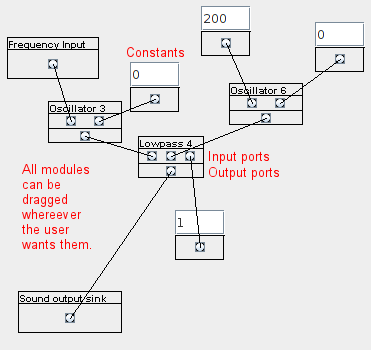
\includegraphics[width=\textwidth]{GUI_cropped}
\end{figure}
A fixed layout could not be used to control a completely free and modular system, so instead I only designed a framework for modules. Most modules (with a few exceptions) are displayed as grey boxes with three rows: The name, the input ports and the output ports. The module box is as small as it can be while fitting all of these together, and the user can drag it anywhere with the mouse, "solving" the problem of layout. Pipes are represented also very minimally, just as a straight line from one port to another. These can be connected by clicking on one port and then on another, and disconnected or reconnected similarly. Right-clicking on the space between modules opens a menu which allows the user to create a new module, or start/stop playing sound. Right-clicking on the module opens up a module-specific options menu. For example, on oscillators this allows the choice of wave function, on the input source allows to create a new note.
The GUI was deliberately kept simple, as it was only a sidelight of this entire project and its purpose was to create an interface to the engine, not be a central aspect for itself. The engine was specifically designed to run separately from the GUI, it would not be difficult to create a completely different interface.


\clearpage

\section{Results}

The resulting software is a stable java program with a GUI interface that allows creating sounds and plays them- Notes can be added manually, and then the exact pathway of the sound can be specified for complete control over the synthesis, before outputting it directly to the standard sound output. 8 types of modules are fully supported, and a few others are coded but are not completely stable or lack a GUI interface (Distortion module, Stereo to Mono splitter). Stereo currently lacks a GUI interface, but the entirety of the engine supports stereo just as well as mono. Polyphony works perfectly, and the amount of free channels can easily be set as a constant when compiling the program.

Future goals would be first and foremost to allow MIDI input, adding more types of modules, polishing the interface and saving. Then support for JACK and external modulation of parameters could be implemented, and finally dedicated editor windows for some of the modules.

\section{Reflection}

\bibliography{references}

\end{document}
